%
% File acl2020.tex
%
%% Based on the style files for ACL 2020, which were
%% Based on the style files for ACL 2018, NAACL 2018/19, which were
%% Based on the style files for ACL-2015, with some improvements
%%  taken from the NAACL-2016 style
%% Based on the style files for ACL-2014, which were, in turn,
%% based on ACL-2013, ACL-2012, ACL-2011, ACL-2010, ACL-IJCNLP-2009,
%% EACL-2009, IJCNLP-2008...
%% Based on the style files for EACL 2006 by 
%%e.agirre@ehu.es or Sergi.Balari@uab.es
%% and that of ACL 08 by Joakim Nivre and Noah Smith

\documentclass[11pt,a4paper]{article}
\usepackage[hyperref]{acl2020}
\usepackage{times}
\usepackage{latexsym}
\renewcommand{\UrlFont}{\ttfamily\small}
\usepackage{graphicx}
% natbib
\bibliographystyle{unsrt}

\usepackage{hyperref}

% This is not strictly necessary, and may be commented out,
% but it will improve the layout of the manuscript,
% and will typically save some space.
\usepackage{microtype}

\aclfinalcopy % Uncomment this line for the final submission
%\def\aclpaperid{***} %  Enter the acl Paper ID here

%\setlength\titlebox{5cm}
% You can expand the titlebox if you need extra space
% to show all the authors. Please do not make the titlebox
% smaller than 5cm (the original size); we will check this
% in the camera-ready version and ask you to change it back.

\newcommand\BibTeX{B\textsc{ib}\TeX}

\title{Fine-tuning and analyzing BERT for resource constrained neural translation}

\author{Shreya Pandit \\
  Department of Computer Science \\
  Boston University \\
  \texttt{shreyap@bu.edu} \\\And
  Alec Hoyland \\
  Center for Systems Neuroscience \\
  Department of Psychological \& Brain Sciences \\
  Boston University \\
  \texttt{ahoyland@bu.edu} \\}

\date{}

\begin{document}
\maketitle
\begin{abstract}
    We trained a \textsc{BERT}-based encoder and Transformer decoder on
    a Neural Translation task between the low resource language Latin
    and English.
    We achieved a \textsc{Bleu} score of 20.23 in comparison to
    our German-English translations which use two high resource languages and achieved a BLEU score of 25.30. We found that the attention mechanism in the encoder correctly attends to the Latin text in a human-interpretable manner
    but noted strong sensitivity to the training corpus' English translations.
    The translations are over a century old
    and this affects the connotation of words used.
    The classical Latin samples are over 2000 years old (for example, the poet Catullus' works are dated between the time period 74BC- 20BC). Despite this, our fine-tuned model was able to leverage non-literal translations to improve clarity in the English translation for modern readers.
\end{abstract}

\section{Introduction}

Automated machine translation is an active field of study in natural language processing. Neural networks currently achieve state-of-the-art in machine translation \citep{ott2019fairseq, tensor2tensor}.
One popular model architecture is the encoder-decoder framework. The encoder embeds a representation of the input text in a high-dimensional vector space. 
The decoder produces a translation output, using the embedded text as input.

Training an encoder-decoder model requires a large bilingual corpus; therefore, trained models are sensitive to the quality and subject matter of the training corpora.
The model is limited by the vocabulary of the corpora and quality of the translation.
This sensitivity is apparent even within corpora from the same language \citep{dellorletta2014linguistic}.
Regardless of architecture, an encoder trained on an English Wikipedia corpus (\href{https://www.english-corpora.org/wiki/}{https://www.english-corpora.org/wiki/}) should be expected to specialize in encoding Standard American English.
This is because the English Wikipedia corpus contains an extremely large (ca. 1.9 billion words) and expansive (ca. 4.4 million articles) sampling of text written in Standard American English.
Training on another corpus would naturally yield different results,
even if the semantic meaning is nearly identical.
For example, if the model were trained on the Simple English Wikipedia instead, a Wikipedia in Standard American English but only using simple words and sentence constructs, we might expect a totally different encoding.

In this paper, we use the pretrained \textsc{Bert} encoder \cite{devlin2018Bert}
and a decoder trained on poetical translations of classical Latin poetry
drawn from The Latin Library (\href{https://thelatinlibrary.com/}{https://thelatinlibrary.com/}).
The corpus was constructed and tokenized using the Classical Language Toolkit (\textsc{cltk}) \cite{johnson2014}.
We explore how training on corpora with the same semantic meaning but different diction influences neural machine translation.

\section{Related Works}

In recent years, neural machine translation (NMT) with deep neural networks has achieved significant improvements over statistical machine translation \citep{DBLP:journals/corr/SutskeverVL14, bahdanau2014neural, cho2014learning}.
In particular, recurrent neural network models have shown success \citep{jozefowicz2016exploring,kuchaiev2017factorization}. 
These models are limited by sequence length, since recurrent neural networks typically generate a sequence of hidden states conditions on the last and the positionally-aligned input.

In contrast, the Transformer architecture disperses with recurrence that relies entirely on an attention mechanism to draw global dependencies between input and output \citep{bahdanau2014neural, vaswani2017attention}.
State-of-the-art in Transformer-based architectures is \textsc{Bert} \citep{devlin2018Bert}.
\textsc{Bert} is a multi-layer bidirectional Transformer encoder with self-attention.
This allows the model to attend to tokens both before and after the current token.
The published model has been pretrained using a masked language model task and a next sentence prediction task, in order to be as general as possible.
\textsc{Bert} was trained using the top 100 language Wikipedia corpora and has been released as a multilanguage model.

Though \textsc{Bert} achieves state-of-the-art results for many language tasks
including reading comprehension and text classification,
the model is not designed specifically for neural machine translation tasks.
Since training \textsc{Bert} is a computationally expensive endeavor,
recent efforts have focused on utilizing the pretrained \textsc{Bert} encoder
on neural machine translation tasks \citep{liu2019text, yang2019making, imamura-sumita-2019-recycling, clinchant2019use}.

Previous work has predominately focused on developing pretraining methods for NMT,
resulting in multiple variants of \textsc{Bert}.
In \textsc{xlm} \citep{lample2019crosslingual},
the model is pretrained on multiple languages without the next-sentence-prediction (NSP) task.
\textsc{RoBERTa} \citep{liu2019roberta} is trained with more unlabeled data and similarly skips the NSP task.
\textsc{XLNet} \citep{yang2019making, dai2019transformerxl}, a permutation-based modeling approach,
introduces a Transformer architecture without fixed-length context.
\textsc{BertViz} is a tool for visualizing attention in Transformer models
\cite{vig2019transformervis}.

\section{Methods}

\subsection{Code Availability Statement}

All source code is freely available at
\href{https://github.com/shreyapandit/bert-nmt-latin}{https://github.com/shreyapandit/bert-nmt-latin}.

\subsection{The \textsc{Bert} model}

\textsc{Bert} makes use of the Transformer architecture,
an attention mechanism that learns contextual relations between tokens.
While the original Transformer model \cite{vaswani2017attention}
includes both an encoder and decoder,
\textsc{Bert} is only a language model
and therefore only includes an encoder mechanism.
Figure \ref{fig:transformer} describes the Transformer architecture,
in which the input sequence is embedded in a high-dimensional output space.
A matching decoder can then decode the embedded sequence into a new language.

The Transformer in \textsc{Bert} is bidirectional,
allowing the model to learn the context of a word based
of its surroundings in both directions (forward and backward).
The \textsc{Bert} model implemented in this paper
is the \textsc{base-multilanguage} model, with 110,000,000 parameters.
\textsc{Bert} was pretrained on 4 cloud tensor-processing units,
using an unsupervised masked language modeling task (Figure \ref{fig:MLM}).
In this task, random tokens in the sequence were obfuscated or mutated.
The model attempted to guess the masked or replaced word.

\begin{figure}
    \centering
    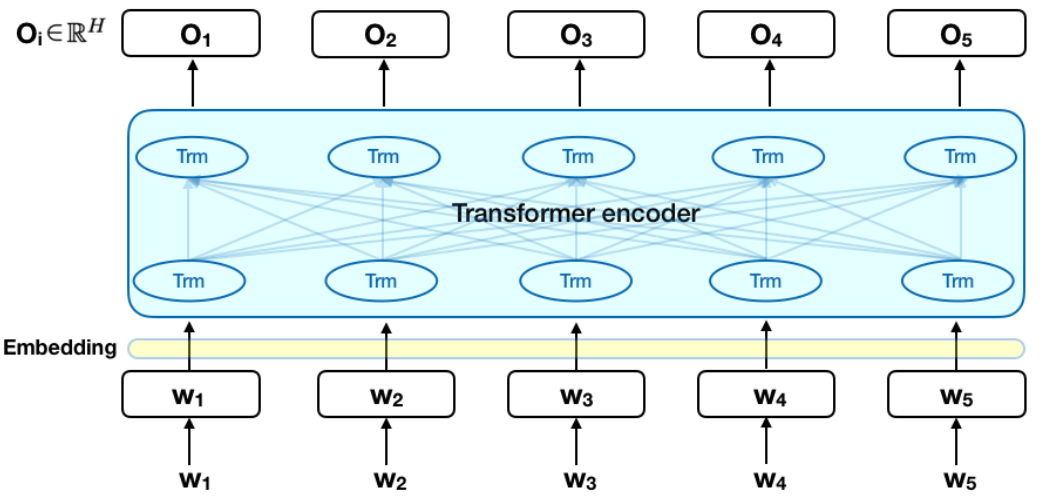
\includegraphics[width=0.4\textwidth]{transformer.png}
    \caption{The Transformer architecture.
    Token representations are embedded in a 768-dimensional space.}
    \label{fig:transformer}
\end{figure}

\begin{figure}
    \centering
    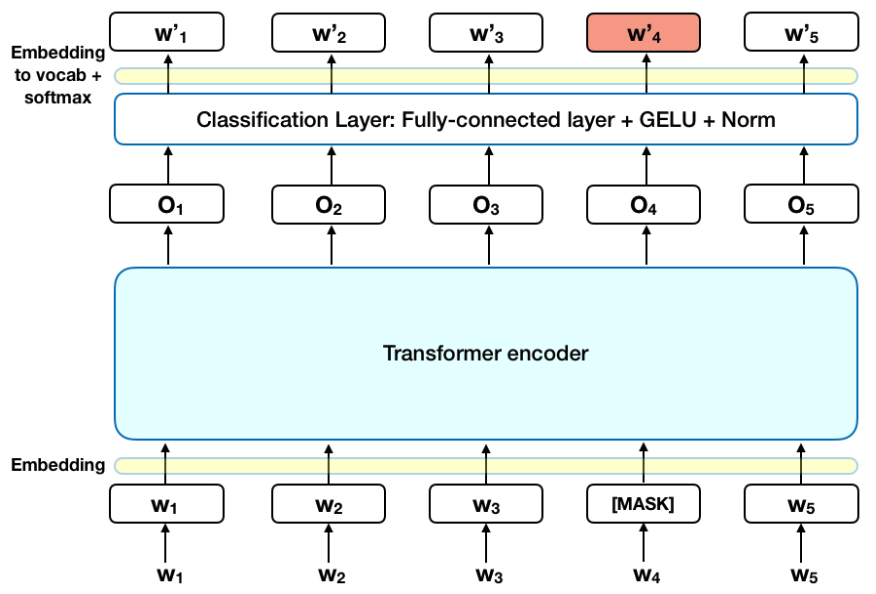
\includegraphics[width=0.4\textwidth]{MLM.png}
    \caption{Schematic of the masked language modeling task
    used to train \textsc{Bert}.
    For machine translation, the classification layer was stripped
    and replaced with a decoder.}
    \label{fig:MLM}
\end{figure}

\subsection{Corpora}

Training data were acquired using the Classical Language Toolkit (\textsc{cltk}) \citep{johnson2014}, from The Latin Library corpus (\href{https://thelatinlibrary.com/}{https://thelatinlibrary.com/}),
comprised of classical Latin texts and verbose, literary translations in English.
\textsc{cltk} lemmatizes and tokenizes using a \textsc{Punkt} tokenizer.
Classical latin does not include punctuation,
however the texts collected at The Latin Library have editorial punctuation.
Therefore, sentence separation was determined by an expert linguist.
The corpus consists of samples of classical Latin writing
with English translations by 19th and 20th century linguists.

The original data were scraped from the Perseus Digital Library at Tufts University
(\href{https://www.perseus.tufts.edu/hopper/}{https://www.perseus.tufts.edu/hopper/})
and compiled in \texttt{.xml} files.
The Latin text was segmented by expert linguists into ``milestones,''
which correspond to sentences or paragraphs in English.
We used the \textsc{BeautifulSoup} Python package
(\href{https://www.crummy.com/software/BeautifulSoup/}{https://www.crummy.com/software/BeautifulSoup/})
to parse xml attributes and content.
We remove markup attributes such as italics and notes
and divide the dataset into training and validation.
These data were saved in a Python data frame,
producing 2,870 samples each consisting of a full sentence or paragraph
from classical Latin texts.

Testing data were compiled by the authors,
one of whom is literate in Latin.
The sentences came from three sources, designed to explore three ``genres'' of Latin literature.
The first includes samples by the neoteric poet Gaius Valerius Catullus.
Each poem is written as a long sentence without punctuation.

The second category is oratory prose, drawn from Marcus Tullius Cicero's Orations Against Catiline.
These sentences are all brief rhetorical questions
which use formal language.

The third category includes samples from an undergraduate Latin I curriculum,
drawn from the first chapter of the textbook, \textit{Ecce Romani} (\href{http://www.tabney.com/ecce1.html}{http://www.tabney.com/ecce1.html}).
In all cases, gold-standard literal translations were provided by the authors.

\begin{table}
        \begin{tabular}{|c | c | } 
        \hline 
        Length of sentence & Proportion of lines \\
        \hline 
        (10, 127]  &  0.634777 \\
        (127, 251]       &          0.279557 \\
        (251, 375]     &            0.064279\\
        (375, 499]    &             0.015708\\
        (499, 624]    &             0.004007\\
        (624, 748]    &             0.001161\\
        (748, 872]    &             0.000293\\
        (872, 996]    &             0.000131\\
        (996, 1120]   &             0.000069\\
        (1120, 1245]  &             0.000019\\
        \hline
    \end{tabular}
    \caption{Distribution of length of German lines in test corpus (normalized).}
    \label{tbl:distde}
\end{table}

\begin{table}
    \begin{tabular}{|c | c | } 
         \hline 
          Length of sentence & Proportion of lines \\
          \hline 
        (19=0, 738]    &  0.960073\\
        (738, 1459]   &   0.028086\\
        (1459, 2180]  &   0.005684\\
        (2180, 2901]  &   0.003131\\
        (2901, 3623]  &   0.000913\\
        (3623, 4344]  &   0.000890\\
        (4344, 5065]  &   0.000659\\
        (6507, 7229]   &  0.000323\\
        (5065, 5786]   &  0.000162\\
        (5786, 6507]   &  0.000081\\
        \hline
    \end{tabular}
    \caption{Distribution of lengths of Latin lines in test corpus (normalized).}
    \label{tbl:distlatin}
\end{table}

Sentences in the Latin corpus were very long.
We split lines with full stop tokens and managed to reduce the skewed distribution.
With longer sentences, we encountered \textsc{cuda} resource allocation errors.
\textsc{Bert} has difficulties with long sequences.
The implementation of \textsc{Bert} limits sequences to 512 tokens and was pretrained on sentence-level representations, meaning that \textsc{Bert} is poorly-optimized for translating long sequences \cite{devlin2018Bert, yang2019making, dai2019transformerxl}.
Increasing the token limit leads to exponential increases in performance time,
so we used the extant hyperparameters of \textsc{Bert} itself as-is.

\begin{table}
    \centering
    \begin{tabular}{| l | r |}
        \hline
        Latin-En Training & 21,544 \\
        Latin-En Testing & 4,063 \\
        De-En Training & 160,239 \\
        De-En Testing & 7,283 \\
        \hline
    \end{tabular}
    \caption{Number of sentences in each dataset}
    \label{tbl:sentences}
\end{table}

\subsection{Training scheme}

Before training, dictionaries were generated from the Latin and English corpora
and the training set was tokenized.
We used \textsc{cltk} to lemmatize and tokenize using a \textsc{Punkt} tokenizer.
Tokens outside the training vocabulary were set to ``Unknown.''

Training was done on an Nvidia Tesla V100 for 100 epochs for both translation (German and Latin) tasks.
Validation was checked after each epoch.
The Adam optimizer was used with a learning rate of 0.001, weight-decay of 0.0001,
and dropout rate of 0.3.
Due to resource limitations and time constraints, we were able to run only a handful of the configuration using a free GPU on Google Colab.
Google Colab provides a V100 during the night and an Nvidia K89 during daytime.
Each run of the model completed within a few hours.

% TODO: Shreya will upload the github link to notebook used to generate Latin dataset

\section{Results}

We used \textsc{BertViz} to visualize the attention of several words using the pretrained multilingual \textsc{Bert} model.
Due to its inflectional syntax, Latin allows for very flexible word ordering.
Despite this, some regularities exist, which can be visualized by observing the attention weights.

For example, the word \textit{quam} has many meanings, including ``in what way,'' ``in comparison to/than,'' however in context with \textit{diu}, the meaning of the word pair becomes ``so long as.''
This expression remains in legal contexts today where it implies ``so long as [good behavior continues].''
\textsc{Bert} pretrained on Latin preserves this meaning, as \textit{quam} strongly attends to \textit{diu} (Figure \ref{fig:quam}).
\textsc{Bert} is also able to capture the meaning of compound words.

The word \textit{etiam} annexes a fact or thought which has already been said.
In general, it means ``and also/furthermore/besides,''
but in the context of time, it means ``still/even now''. 
\textsc{Bert} is able to disambiguate between these meanings,
since \textit{etiam} attends to words indicating temporal context (Figure \ref{fig:etiam}).

In addition, \textsc{Bert} can handle rhetorical ``doubling'' of words,
such as when \textit{iste} (``that'') is used in a pejorative context along with other pronouns.
While it refers to the \textit{furor} (``madness'') of the target of this vitriol (the scheming Lucius Catiline), 
\textsc{Bert} is able to recognize that \textit{tuus} (``your/yours'') has a similar meaning in context, 
resulting in the phrase ``that madness of yours'' (Figure \ref{fig:iste}).

\begin{figure}
  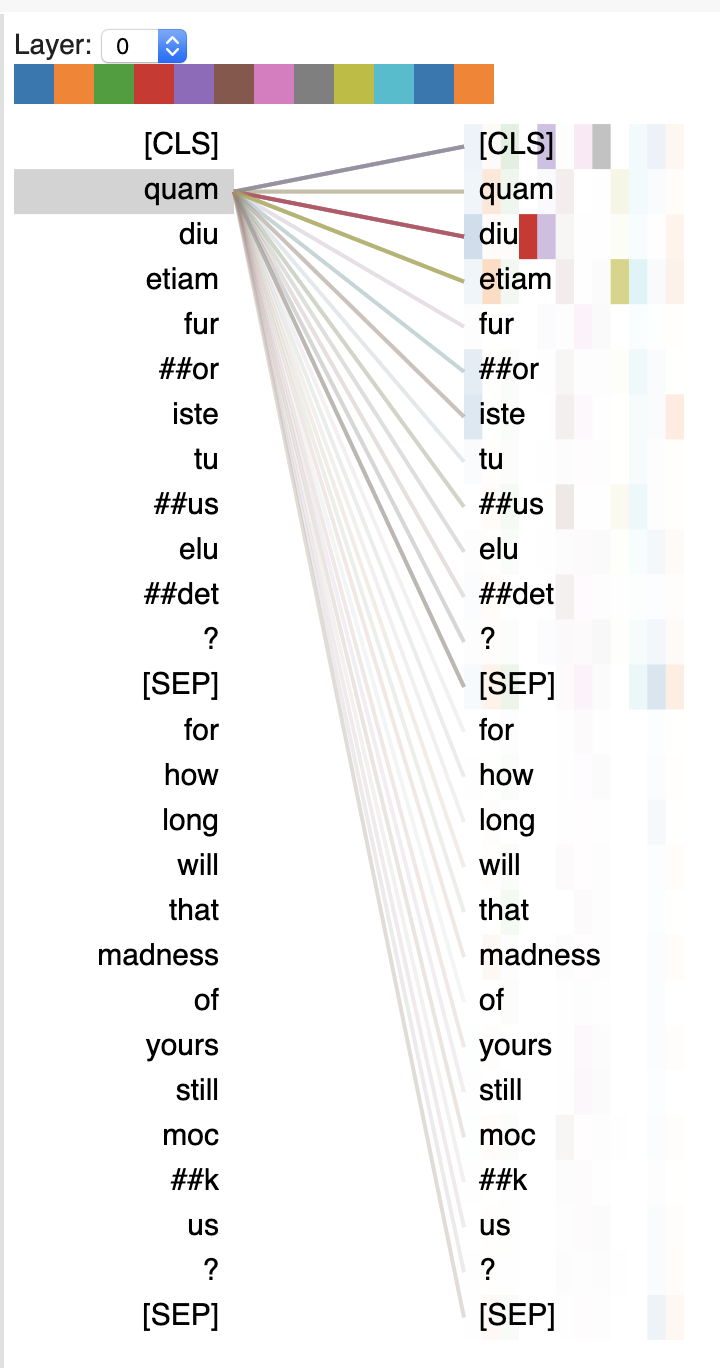
\includegraphics[height=10cm,width=\linewidth,keepaspectratio]{bert-viz/bertviz-quam.png}
  \caption{Attention of word \textit{quam} using bertviz}
  \label{fig:quam}
\end{figure}

\begin{figure}
  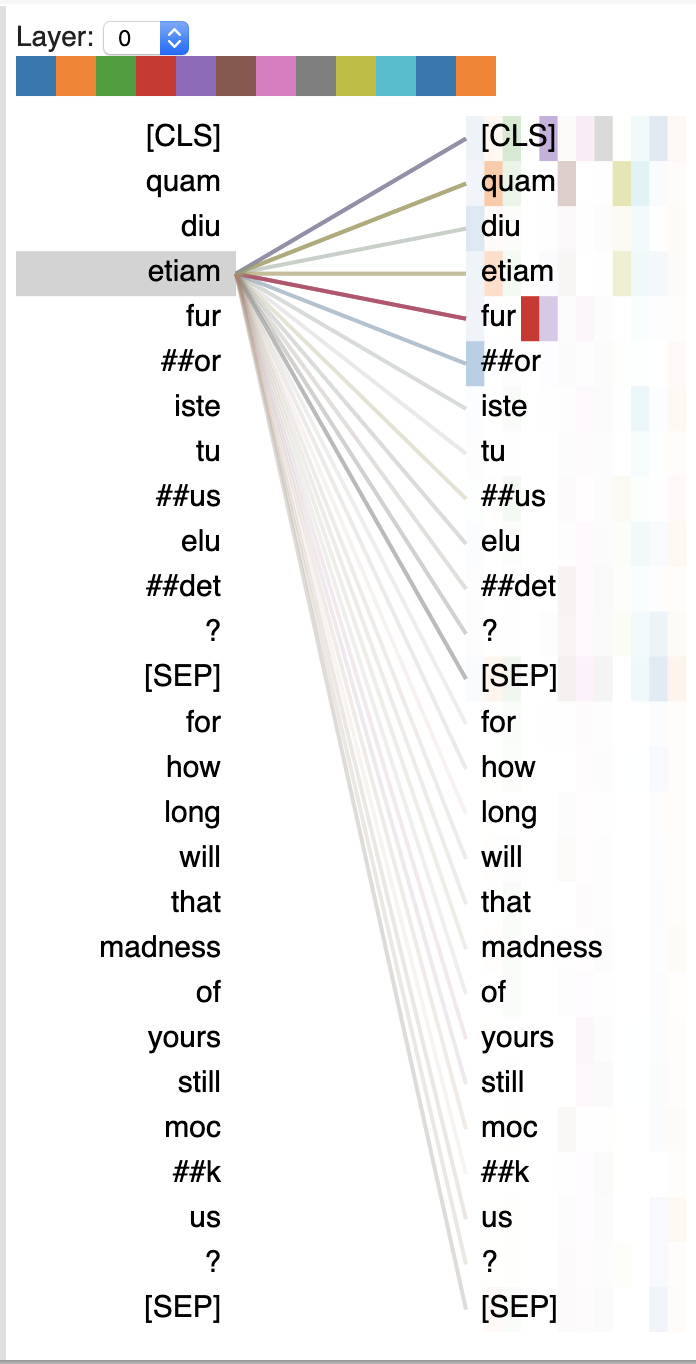
\includegraphics[height=10cm,width=\linewidth,keepaspectratio]{bert-viz/bertviz-etiam.png}
  \caption{Attention of word \textit{etiam} using bertviz}
  \label{fig:etiam}
\end{figure}
\begin{figure}
  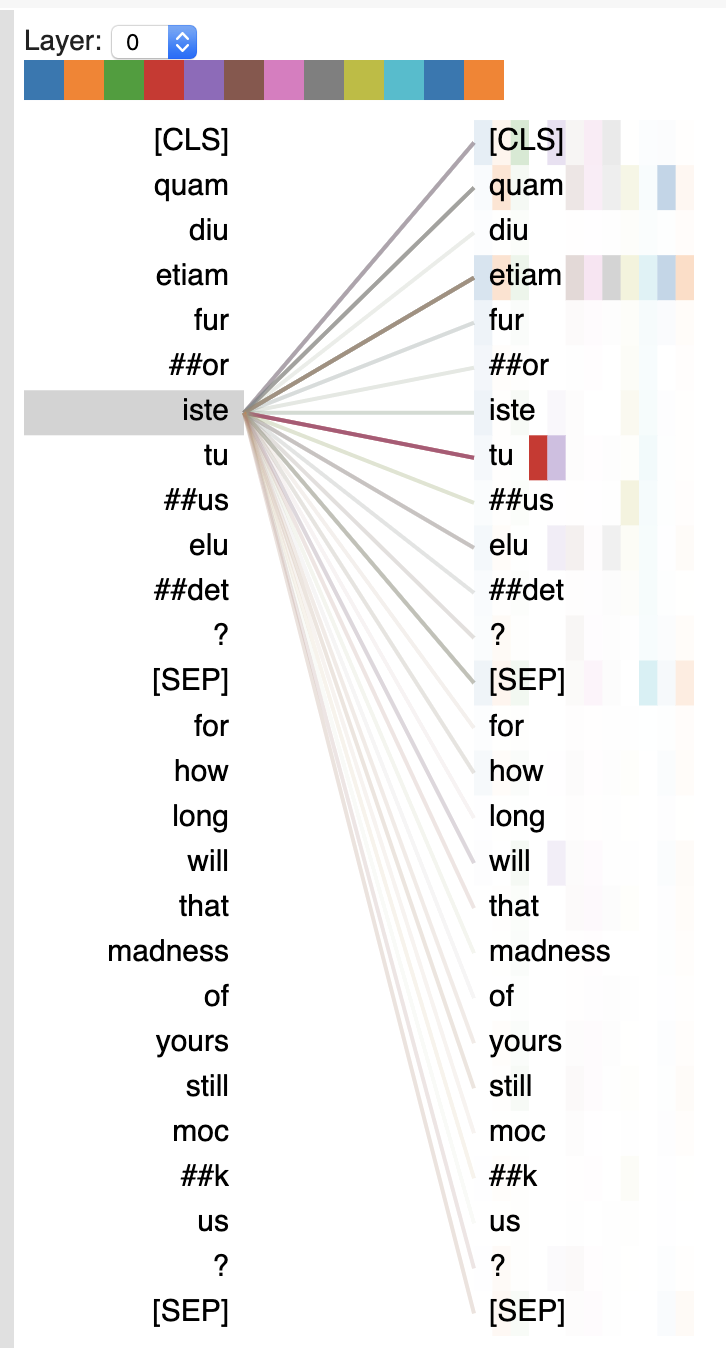
\includegraphics[height=10cm,width=\linewidth,keepaspectratio]{bert-viz/bertviz-iste.png}
  \caption{Attention of word \textit{iste} using bertviz}
  \label{fig:iste}
\end{figure}

We report \textsc{Bleu} scores \cite{papineni-etal-2002-bleu} for the German and Latin translation tasks (Table \ref{tbl:bleu}).

\begin{table}
    \centering
    \begin{tabular}{l | r}
    \hline
    \textsc{Bleu} (De-En) & 25.3  \\
    \textsc{Bleu} (Lat-En) & 20.23 \\
    \hline
    \end{tabular}
    \caption{\textsc{Bleu} scores for the translation tasks.}
    \label{tbl:bleu}
\end{table}

\begin{table}[]
    \centering
    \begin{tabular}{l | r}
        \hline
        Language Pair & Dict. Tokens \\
        \hline
        De-En & 105,878 \\
        Lat-En & 8,368 \\
        \hline
    \end{tabular}
    \caption{Total number of dictionary tokens generated for the two translation tasks.}
    \label{tbl:dict}
\end{table}

\subsection{Examples of translations}

The model perform adequately in translating Latin sentences.
It performed especially well on shorter phrases.
For example,

\begin{quote}
    \textit{de parsimonia ac de pudicitia sua memoratissimus}
\end{quote}

was correctly translated as

\begin{quote}
    regarding his frugality and continence
\end{quote}

It is important to note that non-standard English words were used in the translation.
In common parlance, ``continence'' is generally used in a medical context, to mean the voluntary control of bodily functions.
However, \textit{The Century Dictionary}, published in 1911,
defines ``continence`` as ``moderation or self-restraint.`
This definition much more closely matches with the gold-standard meaning of \textit{pudicitia}, meaning ``chastity, shamefacedness, or modesty.''
Here we see a clear example of how a model trained on formal, academic translations of Latin from the turn of the century affects its ability to translate.

The attention mechanism built into the model is very powerful.
For example, the word \textit{agmen} usually means
a ``train`` or ``flock`` of something,
but can also mean a disordered marching column of soldiers.

\begin{quote}
    \textit{[UNK]is auditis laudatoque suasore et iusso ducere qua n[UNK] agmina cuncta ab institute itinere conversa prae vium sequebantur.}
\end{quote}

is translated as

\begin{quote}
    When this proposition had been heard and its author commended and bidden to lead them by the way that he knew, the whole army changed its intended line of march and followed its guide.
\end{quote}

The conjugated form \textit{agmina} is the plural.
Here, the model correctly identified that
while \textit{agmina} is being used in its military sense,
that the plural ``armies'' is not a good translation in English.
This is because the Roman understanding of an army
is much less unified than the modern definition.
The model opted to translate \textit{agmina} as ``whole army''
to preserve the idea that while they are marching in different columns,
that they are part of the same organization.
This translation is not literal,
but it is more explicable to an English reader
not versed in classical Roman history.

\section{Model Weakness and our implemented improvement}
\subsection{Poor performance on low resource classical dataset}
\begin{itemize}
    \item The BERT multilingual model we implemented as a baseline performed very poorly on sentences of medium to longer length, such as those having 250-300 characters. Such sentences are common in poetry across languages. \textbf{The BLEU scores achieved running the baseline model on sentences of length more than 300 characters were under 1.0}
    \item We can attribute this to the way BERT calculates embeddings. BERT seeks to provide a pre trained method for obtaining contextualized word embeddings for each word of our corpus. It is able to do so by training on sentence pairs and predicting masked words in the input. While this approach may lead BERT to recognize certain subtleties regarding different meaning of a word, it doesn't take into account the sentence length (which might affect the word embeddings)
\end{itemize}

\subsection{Our approach to solve this issue}
\begin{itemize}
    \item We filtered the training data to be a subset of the corpus that had less than 300 characters per sentence. We had 21,554 such training sentences in Latin. These sentences now had 40 tokens on average. \textbf{We fine-tuned BERT embeddings using these and the translations we achieved a BLEU score of 20.23}
    \item We also tried to construct our training corpus in a different way, such as trying to separate Latin milestones using punctuation symbols like ".", however this improved the BLUE score only marginally further than what we achieved using shorter sentences as described above. This approach needs further tweaking because Latin does not have the classical punctuation style as English.
\end{itemize}

\section{Conclusion}

We trained a \textsc{Bert}-based encoder and Transformer decoder on
a translation task between the low resource language Latin
and English.
We achieved a \textsc{Bleu} score of 20.23 in comparison to
our German-English translations which used two high resource languages.
We found that the attention mechanism in the encoder correctly attends to the Latin text in a human-interpretable manner
but noted strong sensitivity to the training corpus' English translations.
The translations are over a century old
and this affects the connotation of words used.
Despite this, the classical Latin samples are over 2000 years old (for example, the poet Catullus' works are dated between the time period 74BC- 20BC)
and the model was able to leverage non-literal translations to improve clarity in the English translation for modern readers.

In addition, we performed experiments to check how different sequence length in the training data affects model performance. We noticed very poor BLEU scores when the tokens per training sample was high (~close to 100). We tried various approaches to overcome this issue, such as filtering on sequences of shorter length, and using punctuation as a baseline to separate training samples. Our improvements over the original Latin training corpus structure improved the BLEU score to 20.23, which is comparable to the BLEU scores achieved for high resource language pairs such as German-English (25.3).

For this paper, we limited our training corpus to only classical Latin rhetoric, poetry, and histories.
We could consider adding translations of the Bible,
however Late Latin and Classical Latin are not perfectly compatible.


We believe that the model can also be improved by tuning model hyperparameters using approaches like Bayesian optimization \cite{snoek2015scalable} and Hyperopt \cite{bergstra2015hyperopt}.

\bibliography{acl2020}

\end{document}
